% L01_full.tex -- Lecture 1: Fintech Foundations and Overview (Full Variant)
% Frames: 31 | Charts: 12 \includegraphics | Arc: 10-role
% Generated for: Financial Technology (FinTech) -- MSc Course, Spring 2026
\documentclass[aspectratio=169, 11pt]{beamer}

% ============================================================
% THEME BASE
% ============================================================
\usetheme{Madrid}
\usecolortheme{whale}

% ============================================================
% PACKAGES
% ============================================================
\usepackage[T1]{fontenc}
\usepackage[utf8]{inputenc}
\usepackage{graphicx}
\usepackage{booktabs}
\usepackage{tikz}
\usepackage{pgfplots}
\usepackage{amsmath}
\usepackage{hyperref}
\usepackage{multicol}
\usepackage{xcolor}

% ============================================================
% TIKZ LIBRARIES
% ============================================================
\usetikzlibrary{arrows.meta, positioning, shapes.geometric, calc, decorations.pathmorphing}

% ============================================================
% PGFPLOTS COMPATIBILITY
% ============================================================
\pgfplotsset{compat=1.18}

% ============================================================
% COLOR DEFINITIONS (Fintech V4 Palette)
% ============================================================
\definecolor{MLPURPLE}{HTML}{9467BD}
\definecolor{MLBLUE}{HTML}{1F77B4}
\definecolor{MLRED}{HTML}{D62728}
\definecolor{MLORANGE}{HTML}{FF7F0E}
\definecolor{MLGREEN}{HTML}{2CA02C}
\definecolor{MLGRAY}{HTML}{7F7F7F}
\definecolor{MLTEAL}{HTML}{0D7377}
\definecolor{MLCYAN}{HTML}{14BDEB}

% Lowercase aliases for use in \textcolor{}
\colorlet{mlpurple}{MLPURPLE}
\colorlet{mlblue}{MLBLUE}
\colorlet{mlred}{MLRED}
\colorlet{mlorange}{MLORANGE}
\colorlet{mlgreen}{MLGREEN}
\colorlet{mlgray}{MLGRAY}
\colorlet{mlteal}{MLTEAL}
\colorlet{mlcyan}{MLCYAN}

% ============================================================
% BEAMER COLOR CUSTOMIZATION
% ============================================================
\setbeamercolor{structure}{fg=MLTEAL}
\setbeamercolor{palette primary}{bg=MLTEAL, fg=white}
\setbeamercolor{palette secondary}{bg=MLTEAL!80, fg=white}
\setbeamercolor{palette tertiary}{bg=MLTEAL!60, fg=white}
\setbeamercolor{palette quaternary}{bg=MLTEAL!40, fg=white}
\setbeamercolor{frametitle}{bg=MLTEAL!10, fg=MLTEAL}
\setbeamercolor{frametitle right}{bg=MLTEAL!5}
\setbeamercolor{block title}{bg=MLTEAL, fg=white}
\setbeamercolor{block body}{bg=MLTEAL!8, fg=black}
\setbeamercolor{block title alerted}{bg=MLRED, fg=white}
\setbeamercolor{block body alerted}{bg=MLRED!8, fg=black}
\setbeamercolor{block title example}{bg=MLGREEN, fg=white}
\setbeamercolor{block body example}{bg=MLGREEN!8, fg=black}
\setbeamercolor{title}{fg=white}
\setbeamercolor{subtitle}{fg=MLCYAN}
\setbeamercolor{author}{fg=white}
\setbeamercolor{institute}{fg=white}
\setbeamercolor{date}{fg=white}
\setbeamercolor{title page header}{bg=MLTEAL}

% ============================================================
% NAVIGATION AND FOOTLINE
% ============================================================
\setbeamertemplate{navigation symbols}{}

\setbeamertemplate{footline}{%
  \leavevmode%
  \hbox{%
    \begin{beamercolorbox}[wd=.333\paperwidth, ht=2.25ex, dp=1ex, center]{palette primary}%
      \usebeamerfont{author in head/foot}\insertshortauthor
    \end{beamercolorbox}%
    \begin{beamercolorbox}[wd=.334\paperwidth, ht=2.25ex, dp=1ex, center]{palette secondary}%
      \usebeamerfont{title in head/foot}\insertshorttitle
    \end{beamercolorbox}%
    \begin{beamercolorbox}[wd=.333\paperwidth, ht=2.25ex, dp=1ex, right]{palette tertiary}%
      \usebeamerfont{date in head/foot}%
      \insertframenumber{} / \inserttotalframenumber\hspace*{2ex}
    \end{beamercolorbox}%
  }%
  \vskip0pt%
}

% ============================================================
% BOTTOM NOTE COMMAND
% ============================================================
\newcommand{\bottomnote}[1]{%
  \vfill
  \begin{beamercolorbox}[wd=\textwidth, ht=2ex, dp=1ex]{palette primary}%
    \tiny\hspace{1em}#1
  \end{beamercolorbox}%
}

% ============================================================
% GRAPHICS PATH
% ============================================================
\graphicspath{{figures/}}

% ============================================================
% COURSE METADATA
% ============================================================
\title{Financial Technology (FinTech)}
\author{Joerg Osterrieder}
\institute{University of Zurich \\ Department of Finance}
\date{Spring 2026}


\subtitle{Understanding the Revolution in Financial Services}

\begin{document}

% =============================================================================
% === WHY === (Frames 1--4: Title, Opening Cartoon, Learning Objectives, Bridge)
% =============================================================================

% --- Frame 1: Title Page ---
\begin{frame}{Title Page}
  \titlepage
\end{frame}

% --- Frame 2: Opening Cartoon ---
\begin{frame}{The Fintech Disruption}
  \begin{center}
    \includegraphics[width=0.85\textwidth]{11_opening_cartoon/cartoon.pdf}
  \end{center}
  \vspace{-0.5em}
  \begin{center}
    \textit{``The revolution started in a garage, not a boardroom.''}
  \end{center}
  \bottomnote{This is the tension at the heart of fintech: speed vs.\ scale, innovation vs.\ regulation.}
\end{frame}

% --- Frame 3: Learning Objectives ---
\begin{frame}{Learning Objectives}
  By the end of this lecture you will be able to:
  \begin{enumerate}
    \item \textbf{Describe} the defining characteristics of fintech and trace its
          historical evolution from early electronic banking to modern embedded
          finance. \hfill\textit{[Understand]}
    \item \textbf{Explain} how the 2008 financial crisis acted as a catalyst for
          fintech innovation by eroding trust in traditional institutions.
          \hfill\textit{[Understand]}
    \item \textbf{Classify} the major collaboration models between traditional
          financial institutions and fintech companies. \hfill\textit{[Apply]}
    \item \textbf{Compare} the competitive advantages and disadvantages of
          incumbent banks vs.\ fintech startups across key service dimensions.
          \hfill\textit{[Analyze]}
    \item \textbf{Evaluate} which collaboration model best fits a given strategic
          scenario. \hfill\textit{[Evaluate]}
  \end{enumerate}
  \vspace{0.5em}
  \textcolor{mlpurple}{\textbf{Bloom's levels covered:}} Understand, Apply, Analyze, Evaluate
  \bottomnote{These objectives map directly to quiz and exercise assessments.}
\end{frame}

% --- Frame 4: Bridge / Welcome ---
\begin{frame}{Welcome to Financial Technology}
  \begin{columns}[T]
    \begin{column}{0.55\textwidth}
      Welcome to Financial Technology.

      \vspace{0.5em}
      This course examines how technology is transforming every corner of
      financial services --- from payments and lending to insurance and wealth
      management.

      \vspace{0.5em}
      This first lecture establishes the foundation:
      \begin{itemize}
        \item What fintech \textbf{is}
        \item Where it \textbf{came from}
        \item Where it is \textbf{going}
      \end{itemize}
    \end{column}
    \begin{column}{0.42\textwidth}
      \includegraphics[width=\textwidth]{04_fintech_ecosystem_overview/chart.pdf}
    \end{column}
  \end{columns}
  \bottomnote{By the end of this lecture you will have a framework for understanding every topic in the rest of the course.}
\end{frame}

% =============================================================================
% === FEEL === (Frame 5: Personal Connection)
% =============================================================================

% --- Frame 5: The Fintech in Your Pocket ---
\begin{frame}{The Fintech in Your Pocket}
  Think about the last 48 hours.

  \vspace{0.5em}
  How many financial transactions did you make? How many involved a traditional
  bank branch? Now open your phone --- how many apps touch your money? Banking,
  payments, investment, insurance? \textcolor{mlpurple}{Each one is a fintech story.}

  \vspace{0.8em}
  \begin{exampleblock}{Quick Exercise}
    Count the financial apps on your phone. For each, ask:
    \begin{itemize}
      \item Is this from a \textbf{traditional bank}, a \textbf{fintech startup},
            or a \textbf{big tech company}?
    \end{itemize}
    Bring your count to the discussion.
  \end{exampleblock}
  \bottomnote{Most MSc students have 5--10 financial apps --- and most are NOT from their bank.}
\end{frame}

% =============================================================================
% === WHAT === (Frames 6--9: Foundational Concepts)
% =============================================================================

% --- Frame 6: What Is Fintech? ---
\begin{frame}{What Is Fintech? Definitions Across Perspectives}
  \begin{columns}[T]
    \begin{column}{0.55\textwidth}
      \begin{tabular}{@{}l p{4.8cm}@{}}
        \toprule
        \textbf{Perspective} & \textbf{Definition Focus} \\
        \midrule
        Academic   & Technology-enabled financial innovation \\
        Industry   & Companies using tech to improve financial services \\
        Regulatory & New entrants requiring new oversight frameworks \\
        Consumer   & Faster, cheaper, more accessible financial products \\
        \bottomrule
      \end{tabular}
    \end{column}
    \begin{column}{0.42\textwidth}
      Notice: every definition emphasizes a different stakeholder.

      \vspace{0.4em}
      Academics see \textit{innovation}. Industry sees \textit{competition}.
      Regulators see \textit{risk}. Consumers see \textit{convenience}.

      \vspace{0.4em}
      \textcolor{mlpurple}{Fintech is all four simultaneously.}
    \end{column}
  \end{columns}
  \vspace{0.5em}
  \begin{block}{Working Definition}
    Fintech is not a product --- it is a force that reshapes how financial
    services are created, delivered, and consumed.
  \end{block}
  \bottomnote{The term `fintech' was first used in the early 1990s but gained mainstream adoption after 2010.}
\end{frame}

% --- Frame 7: The Scope of Fintech ---
\begin{frame}{The Scope of Fintech --- Seven Verticals}
  \begin{enumerate}
    \item \textcolor{mlpurple}{\textbf{Payments}} --- mobile wallets, real-time transfers, cross-border
    \item \textcolor{mlpurple}{\textbf{Lending}} --- peer-to-peer, alternative credit scoring, BNPL
    \item \textcolor{mlpurple}{\textbf{Insurance (Insurtech)}} --- on-demand, parametric, automated claims
    \item \textcolor{mlpurple}{\textbf{Wealth Management}} --- robo-advisors, micro-investing, social trading
    \item \textcolor{mlpurple}{\textbf{Capital Markets}} --- algorithmic trading, tokenization, crowdfunding
    \item \textcolor{mlpurple}{\textbf{RegTech}} --- compliance automation, identity verification, monitoring
    \item \textcolor{mlpurple}{\textbf{Banking Infrastructure}} --- neobanks, BaaS, open banking APIs
  \end{enumerate}
  \vspace{0.3em}
  \begin{block}{Course Roadmap}
    Each vertical is a lecture in this course. Today we see the forest; later we
    examine each tree.
  \end{block}
  \bottomnote{Lectures 3--7 each deep-dive into one or more of these verticals.}
\end{frame}

% --- Frame 8: Timeline of Financial Innovation ---
\begin{frame}{From Abacus to Algorithm --- A Timeline of Financial Innovation}
  \begin{center}
    \includegraphics[width=0.88\textwidth]{01_fintech_evolution_timeline/chart.pdf}
  \end{center}
  \vspace{-0.3em}
  \begin{itemize}
    \item \textbf{What you see:} Major fintech milestones from the 1950s to the
          2020s --- credit cards, ATMs, online banking, mobile payments,
          blockchain, embedded finance.
    \item \textbf{Key pattern:} The pace of innovation \textit{accelerates}. The
          gap between credit cards and ATMs was a decade; between mobile payments
          and blockchain, just years.
    \item \textbf{Takeaway:} Each wave builds on the infrastructure of the
          previous one.
  \end{itemize}
  \bottomnote{The timeline is illustrative. Exact dates vary by region --- ATMs arrived in the US in 1969 but in many developing countries decades later.}
\end{frame}

% --- Frame 9: Traditional Banking vs. Fintech ---
\begin{frame}{Traditional Banking vs.\ Fintech --- What Changed?}
  \begin{center}
    \includegraphics[width=0.85\textwidth]{02_banking_value_chain_disruption/chart.pdf}
  \end{center}
  \vspace{-0.3em}
  \begin{itemize}
    \item \textbf{What you see:} The traditional bank as a vertically integrated
          institution vs.\ specialized fintechs attacking each layer.
    \item \textbf{Key pattern:} Fintech does not replace the bank. It
          \textit{unbundles} it --- each startup attacks the most profitable or
          most inefficient piece.
    \item \textbf{Takeaway:} The question is not ``Will banks disappear?'' but
          ``Which parts of banking can survive unbundling?''
  \end{itemize}
  \bottomnote{This unbundling-rebundling cycle is the central dynamic of fintech disruption. See L02 for ecosystem analysis.}
\end{frame}

% =============================================================================
% === CASE === (Frames 10--13: The Great Recession Catalyst)
% =============================================================================

% --- Frame 10: Before 2008 ---
\begin{frame}{Before 2008 --- The Trust Assumption}
  \begin{columns}[T]
    \begin{column}{0.50\textwidth}
      Before the crisis, the banking landscape was stable and predictable:

      \vspace{0.5em}
      \begin{itemize}
        \item High trust in institutions
        \item Limited alternatives for consumers
        \item Regulatory frameworks designed for incumbents
        \item Innovation happened \textit{inside} banks, not outside
      \end{itemize}
    \end{column}
    \begin{column}{0.47\textwidth}
      \vspace{0.5em}
      Banks were the only game in town. Consumers trusted them by default.
      Regulation protected them from competition. Innovation meant a new
      savings product, not a new business model.

      \vspace{0.5em}
      \begin{alertblock}{Key Insight}
        Trust in banks was not earned --- it was \textbf{assumed}. The crisis
        exposed the assumption.
      \end{alertblock}
    \end{column}
  \end{columns}
  \bottomnote{In 2007, over 80\% of consumers in developed markets expressed high trust in their primary bank.}
\end{frame}

% --- Frame 11: Trust Collapses ---
\begin{frame}{The 2008 Crisis --- Trust Collapses}
  \begin{center}
    \includegraphics[width=0.82\textwidth]{05_great_recession_catalyst/chart.pdf}
  \end{center}
  \vspace{-0.3em}
  \begin{itemize}
    \item \textbf{What you see:} A causal chain from the housing bubble to the
          opening of space for fintech entrants.
    \item \textbf{Key pattern:} Each step reduced a barrier to fintech entry.
          Trust erosion created \textit{demand}. Regulatory response created
          \textit{opportunity}. Unemployment created \textit{talent supply}.
    \item \textbf{Takeaway:} The 2008 crisis did not cause fintech, but it
          \textcolor{mlpurple}{removed the barriers} that had held it back for
          decades.
  \end{itemize}
  \bottomnote{By 2010, trust in banks had fallen to historic lows in the US, UK, and Eurozone.}
\end{frame}

% --- Frame 12: Three Forces ---
\begin{frame}{Three Forces That Opened the Door}
  \begin{columns}[T]
    \begin{column}{0.31\textwidth}
      \begin{block}{Demand Shift}
        Consumers, especially millennials, sought alternatives to banks they no
        longer trusted.

        \vspace{0.3em}
        Digital-native expectations: speed, transparency, mobile-first.
      \end{block}
    \end{column}
    \begin{column}{0.31\textwidth}
      \begin{block}{Regulatory Response}
        Post-crisis regulation (Dodd-Frank, PSD2, Open Banking) inadvertently
        created space for non-bank competitors.

        \vspace{0.3em}
        Regulatory sandboxes invited startups.
      \end{block}
    \end{column}
    \begin{column}{0.31\textwidth}
      \begin{block}{Technology + Talent}
        Cloud computing reduced infrastructure costs. Smartphones created
        distribution channels.

        \vspace{0.3em}
        Laid-off bankers became fintech founders.
      \end{block}
    \end{column}
  \end{columns}
  \vspace{0.5em}
  \begin{center}
    \textcolor{mlpurple}{\textbf{Fintech needed all three forces simultaneously.
    Technology alone was not enough --- it needed demand and regulatory permission.}}
  \end{center}
  \bottomnote{The smartphone was necessary but not sufficient. The crisis provided the push; the technology provided the path.}
\end{frame}

% --- Frame 13: Post-Crisis Boom ---
\begin{frame}{Post-Crisis Fintech Boom --- The Numbers}
  \begin{center}
    \includegraphics[width=0.82\textwidth]{06_fintech_investment_growth/chart.pdf}
  \end{center}
  \vspace{-0.3em}
  \begin{itemize}
    \item After 2010, venture capital flooded into fintech.
    \item Initial investments were small (seed/Series~A); by 2020, fintech
          companies were raising \textcolor{mlpurple}{billions}.
    \item The pandemic in 2020 further accelerated digital adoption.
  \end{itemize}
  \bottomnote{Investment data is illustrative of the growth trajectory. Actual figures vary by source and definition of `fintech'.}
\end{frame}

% =============================================================================
% === HOW === (Frames 14--17: Collaboration Models)
% =============================================================================

% --- Frame 14: The Collaboration Spectrum ---
\begin{frame}{The Collaboration Spectrum --- From Competition to Partnership}
  \begin{center}
    \includegraphics[width=0.82\textwidth]{03_collaboration_models_matrix/chart.pdf}
  \end{center}
  \vspace{-0.3em}
  \begin{itemize}
    \item \textbf{What you see:} Four models for how banks and fintechs work
          together, scored across five dimensions.
    \item \textbf{Key pattern:} No single model dominates. Partnerships offer
          speed but less control. Acquisitions offer control but are expensive
          and slow.
    \item \textbf{Takeaway:} The ``right'' model depends on the bank's strategic
          priorities and the fintech's maturity.
  \end{itemize}
  \bottomnote{Most large banks use multiple models simultaneously --- partnering in payments, acquiring in lending, building white-label for compliance.}
\end{frame}

% --- Frame 15: Partnership Model ---
\begin{frame}{Partnership Model --- How It Works}
  \begin{columns}[T]
    \begin{column}{0.52\textwidth}
      \includegraphics[width=\textwidth]{07_bank_fintech_partnership_flow/chart.pdf}
    \end{column}
    \begin{column}{0.45\textwidth}
      Partnerships are the most common model.

      \vspace{0.4em}
      The \textbf{bank} brings what it has:
      \begin{itemize}
        \item Banking license
        \item Customer base
        \item Capital \& compliance
      \end{itemize}

      \vspace{0.3em}
      The \textbf{fintech} brings what it does better:
      \begin{itemize}
        \item Technology platform
        \item User experience
        \item Speed \& innovation
      \end{itemize}

      \vspace{0.3em}
      \begin{block}{Success Criterion}
        A partnership succeeds when each party contributes something the other
        cannot build faster alone.
      \end{block}
    \end{column}
  \end{columns}
  \bottomnote{Examples: Goldman Sachs + Apple (Apple Card), JPMorgan + OnDeck (small business lending), BBVA + Atom Bank.}
\end{frame}

% --- Frame 16: Acquisition and White-Label ---
\begin{frame}{Acquisition and White-Label --- Two More Paths}
  \begin{columns}[T]
    \begin{column}{0.47\textwidth}
      \begin{block}{Acquisition}
        Bank buys fintech outright. Gains technology and talent.

        \vspace{0.3em}
        \textcolor{mlred}{\textbf{Risk:}} Culture clash kills innovation. The
        acquired team leaves.

        \vspace{0.3em}
        \textit{Pattern:} Large bank buys Series~B fintech for technology stack.
      \end{block}
    \end{column}
    \begin{column}{0.47\textwidth}
      \begin{block}{White-Label / BaaS}
        Fintech builds infrastructure; bank puts its brand on top.

        \vspace{0.3em}
        Banking-as-a-Service (BaaS). The fintech is \textbf{invisible} to the
        consumer.

        \vspace{0.3em}
        \textit{Pattern:} Neobank runs on a licensed bank's infrastructure.
      \end{block}
    \end{column}
  \end{columns}
  \vspace{0.5em}
  \begin{alertblock}{Three Paths Compared}
    Acquisition buys the \textit{past}. White-label rents the \textit{present}.
    Partnership builds the \textit{future}.
  \end{alertblock}
  \bottomnote{White-label and BaaS are growing fastest. They let banks innovate without building, and fintechs scale without a license.}
\end{frame}

% --- Frame 17: Open Banking ---
\begin{frame}{Open Banking --- The Regulatory Path}
  \begin{columns}[T]
    \begin{column}{0.52\textwidth}
      \textbf{Open banking} is a regulatory mandate requiring banks to share
      customer data via APIs with authorized third parties.

      \vspace{0.5em}
      Key regulations:
      \begin{itemize}
        \item \textbf{PSD2} (EU, 2018)
        \item \textbf{Open Banking Standard} (UK)
        \item \textbf{PIX} (Brazil)
        \item \textbf{Account Aggregator} (India)
      \end{itemize}

      \vspace{0.3em}
      Open banking creates a level playing field by turning bank data from a
      \textit{moat} into a \textcolor{mlpurple}{shared resource}.
    \end{column}
    \begin{column}{0.45\textwidth}
      \vspace{0.3em}
      \begin{center}
        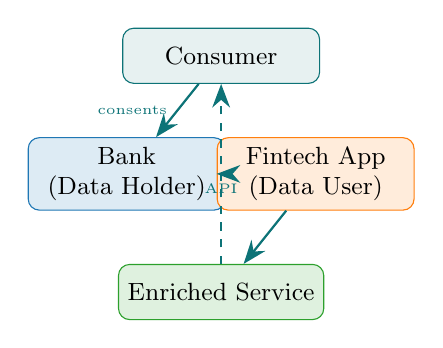
\begin{tikzpicture}[
          box/.style={rectangle, draw=MLTEAL, fill=MLTEAL!10, rounded corners,
                      minimum width=2.5cm, minimum height=0.7cm, align=center,
                      font=\small},
          arr/.style={-{Stealth[length=3mm]}, thick, MLTEAL}
        ]
          \node[box] (consumer) at (0,3) {Consumer};
          \node[box, fill=MLBLUE!15, draw=MLBLUE] (bank) at (-1.2,1.5) {Bank\\(Data Holder)};
          \node[box, fill=MLORANGE!15, draw=MLORANGE] (fintech) at (1.2,1.5) {Fintech App\\(Data User)};
          \node[box, fill=MLGREEN!15, draw=MLGREEN] (service) at (0,0) {Enriched Service};
          \draw[arr] (consumer) -- node[left, font=\tiny] {consents} (bank);
          \draw[arr] (bank) -- node[below, font=\tiny] {API} (fintech);
          \draw[arr] (fintech) -- (service);
          \draw[arr, dashed] (service) -- (consumer);
        \end{tikzpicture}
      \end{center}
    \end{column}
  \end{columns}
  \vspace{0.2em}
  \begin{block}{The Implication}
    Open banking turns the bank's greatest asset --- customer data --- into a
    shared resource. The bank that adapts fastest wins.
  \end{block}
  \bottomnote{PSD2 (EU, 2018) was the first major open banking mandate. The UK's Open Banking Standard, Brazil's PIX, and India's Account Aggregator followed.}
\end{frame}

% =============================================================================
% === RISK === (Frames 18--20: What Can Go Wrong)
% =============================================================================

% --- Frame 18: When Fintech Fails ---
\begin{frame}{When Fintech Fails --- Common Failure Modes}
  \begin{enumerate}
    \item \textcolor{mlred}{\textbf{Regulatory risk}} --- Operating without
          adequate licenses; crossing jurisdictional boundaries without
          authorization.
    \item \textcolor{mlred}{\textbf{Trust risk}} --- Data breaches; lack of
          deposit insurance; unclear complaint resolution pathways.
    \item \textcolor{mlred}{\textbf{Scalability risk}} --- Customer acquisition
          costs exceed lifetime value; unit economics never work at scale.
    \item \textcolor{mlred}{\textbf{Systemic risk}} --- Fintech becomes ``too
          connected to fail''; concentration in a small number of cloud
          providers.
  \end{enumerate}
  \vspace{0.3em}
  \begin{alertblock}{The Bigger Question}
    Fintech disruption is not risk-free. The question is whether fintech creates
    \textit{new} risks or merely redistributes old ones.
  \end{alertblock}
  \bottomnote{See L04 (RegTech and Fintech Regulation) for detailed analysis of regulatory failure modes.}
\end{frame}

% --- Frame 19: Consumer Protection ---
\begin{frame}{The Consumer Protection Challenge}
  \begin{columns}[T]
    \begin{column}{0.50\textwidth}
      Traditional banks are regulated, insured, and supervised.

      \vspace{0.5em}
      Fintech companies often operate in \textcolor{mlred}{regulatory gaps} ---
      between banking law and technology law, between national jurisdictions.
    \end{column}
    \begin{column}{0.47\textwidth}
      Key consumer protection concerns:
      \begin{itemize}
        \item Deposit insurance gaps
        \item Data privacy vulnerabilities
        \item Algorithmic bias in lending
        \item Cross-border enforcement difficulties
      \end{itemize}
    \end{column}
  \end{columns}
  \vspace{0.5em}
  \begin{alertblock}{A Critical Principle}
    Innovation without consumer protection is not progress --- it is
    \textbf{risk transfer} from institutions to individuals.
  \end{alertblock}
  \bottomnote{This tension between innovation and protection is the central theme of L04 (Fintech Security and Regulation).}
\end{frame}

% --- Frame 20: Cybersecurity and Operational Risk ---
\begin{frame}{Cybersecurity and Operational Risk}
  \begin{columns}[T]
    \begin{column}{0.50\textwidth}
      \vspace{-0.5em}
      \begin{tabular}{@{}l l l@{}}
        \toprule
        \textbf{Risk Type} & \textbf{Trad.\ Bank} & \textbf{Fintech} \\
        \midrule
        Data breach  & Internal systems  & Cloud + APIs \\
        Outage       & Redundant infra   & Single cloud \\
        Fraud        & Known patterns    & Novel vectors \\
        Compliance   & Established       & Evolving \\
        \bottomrule
      \end{tabular}
    \end{column}
    \begin{column}{0.47\textwidth}
      Fintech companies often have \textbf{larger attack surfaces} (more APIs,
      more cloud dependencies, more third-party integrations) but
      \textbf{smaller security teams}.

      \vspace{0.5em}
      The trade-off: \textcolor{mlpurple}{speed-to-market} vs.\
      \textcolor{mlred}{security-in-depth}.
    \end{column}
  \end{columns}
  \bottomnote{L07 (Technology of FinTech) covers identity, encryption, and cybersecurity in depth.}
\end{frame}

% =============================================================================
% === WHERE === (Frames 21--23: Evidence at Scale)
% =============================================================================

% --- Frame 21: Regional Patterns ---
\begin{frame}{Fintech Around the World --- Regional Patterns}
  \begin{center}
    \includegraphics[width=0.80\textwidth]{09_fintech_impact_comparison/chart.pdf}
  \end{center}
  \vspace{-0.3em}
  \begin{itemize}
    \item \textbf{What you see:} Fintech adoption varies dramatically by region,
          with Asia-Pacific and Africa leading in mobile payments.
    \item \textbf{Key pattern:} Regions with weaker traditional banking
          infrastructure often \textcolor{mlpurple}{leapfrog} to fintech --- the
          ``leapfrog effect.''
    \item \textbf{Takeaway:} The most transformative fintech innovations
          (M-Pesa, Alipay, PIX) emerged \textit{outside} the US and Europe.
  \end{itemize}
  \bottomnote{Data is illustrative of broad adoption patterns. Actual metrics depend on definition and measurement methodology.}
\end{frame}

% --- Frame 22: Key Trends ---
\begin{frame}{Key Trends Reshaping Fintech}
  \begin{enumerate}
    \item \textcolor{mlpurple}{\textbf{Embedded finance}} --- Financial services
          integrated into non-financial platforms (ride-sharing with payments,
          e-commerce with lending, social media with tipping).
    \item \textcolor{mlpurple}{\textbf{Neobanks}} --- Digital-only banks
          challenging incumbents on user experience and fees.
    \item \textcolor{mlpurple}{\textbf{Decentralized finance (DeFi)}} ---
          Financial services built on blockchain, removing intermediaries.
    \item \textcolor{mlpurple}{\textbf{Super-apps}} --- Single platforms
          combining messaging, payments, shopping, banking (WeChat, Grab,
          Gojek).
    \item \textcolor{mlpurple}{\textbf{Sustainable fintech}} --- Green bonds, ESG
          scoring, carbon-tracking financial products.
  \end{enumerate}
  \vspace{0.3em}
  \begin{block}{Opportunity and Threat}
    Each of these trends is both an opportunity and a threat. The winners will be
    those who combine innovation with trust.
  \end{block}
  \bottomnote{Lectures 3--7 examine these trends in depth. Today we establish the landscape.}
\end{frame}

% --- Frame 23: Three Scenarios ---
\begin{frame}{The Future of Banking --- Three Scenarios}
  \begin{columns}[T]
    \begin{column}{0.31\textwidth}
      \begin{block}{\centering Banks Win}
        Incumbents absorb fintech capabilities through acquisition and internal
        innovation.

        \vspace{0.3em}
        Regulation protects their position.

        \vspace{0.3em}
        \textit{Result:} Banks look different but remain dominant.
      \end{block}
    \end{column}
    \begin{column}{0.31\textwidth}
      \begin{block}{\centering Fintech Wins}
        Startups capture enough market share to become the new incumbents.

        \vspace{0.3em}
        Big tech enters financial services.

        \vspace{0.3em}
        \textit{Result:} Banks become utilities --- infrastructure, not
        customer-facing.
      \end{block}
    \end{column}
    \begin{column}{0.31\textwidth}
      \begin{block}{\centering Coexistence}
        Banks handle regulated activities (deposits, lending); fintechs handle
        customer experience.

        \vspace{0.3em}
        Open banking APIs connect them.

        \vspace{0.3em}
        \textit{Result:} Specialization by comparative advantage.
      \end{block}
    \end{column}
  \end{columns}
  \vspace{0.3em}
  \begin{center}
    \textcolor{mlpurple}{\textbf{The most likely outcome is coexistence --- but
    which segments go to banks vs.\ fintechs will define the next decade.}}
  \end{center}
  \bottomnote{This question recurs throughout the course. Each lecture adds evidence for one scenario or another.}
\end{frame}

% =============================================================================
% === IMPACT === (Frames 24--25: Who Wins, Who Loses)
% =============================================================================

% --- Frame 24: Stakeholder Impact Analysis ---
\begin{frame}{Stakeholder Impact Analysis}
  \begin{columns}[T]
    \begin{column}{0.45\textwidth}
      \includegraphics[width=\textwidth]{08_embedded_finance_architecture/chart.pdf}
    \end{column}
    \begin{column}{0.52\textwidth}
      \begin{itemize}
        \item \textbf{Consumers:} More choice, lower fees --- but less
              protection
        \item \textbf{Banks:} Competitive pressure, forced innovation,
              potential disintermediation
        \item \textbf{Regulators:} New oversight challenges, innovation vs.\
              stability trade-off
        \item \textbf{Fintechs:} Growth opportunity --- but funding cycles and
              regulatory uncertainty
        \item \textbf{Society:} Financial inclusion gains --- but digital
              divide risks
      \end{itemize}
    \end{column}
  \end{columns}
  \vspace{0.3em}
  \begin{block}{Not Zero-Sum}
    Fintech is not zero-sum. Both consumers and institutions can benefit --- but
    the benefits are \textcolor{mlpurple}{not evenly distributed}.
  \end{block}
  \bottomnote{Financial inclusion --- serving the unbanked and underbanked --- is examined in detail in L02 (Fintech Ecosystem).}
\end{frame}

% --- Frame 25: Financial Inclusion ---
\begin{frame}{The Financial Inclusion Promise}
  \begin{columns}[T]
    \begin{column}{0.50\textwidth}
      How fintech enables financial inclusion:

      \vspace{0.5em}
      \begin{itemize}
        \item \textbf{Mobile money} serving unbanked populations
        \item \textbf{Alternative credit scoring} using non-traditional data
        \item \textbf{Micro-investing} lowering entry barriers
        \item \textbf{Cross-border remittances} reducing transfer costs
      \end{itemize}
    \end{column}
    \begin{column}{0.47\textwidth}
      \vspace{0.5em}
      Over \textcolor{mlpurple}{\textbf{1.7~billion}} adults globally lack
      access to formal financial services.

      \vspace{0.5em}
      Fintech's greatest promise is reaching them --- not through branches,
      but through \textbf{smartphones}.
    \end{column}
  \end{columns}
  \vspace{0.5em}
  \begin{exampleblock}{The Litmus Test}
    If fintech only serves the already-served, it is \textit{optimization}, not
    transformation. \textcolor{mlpurple}{Inclusion is the test of genuine impact.}
  \end{exampleblock}
  \bottomnote{M-Pesa (Kenya, 2007) remains the canonical example. See L02 for the full financial inclusion discussion.}
\end{frame}

% =============================================================================
% === SO WHAT === (Frames 26--27: Synthesis and Evaluation)
% =============================================================================

% --- Frame 26: Five Questions Framework ---
\begin{frame}{Five Questions That Reveal Any Fintech's True Strategy}
  \begin{columns}[T]
    \begin{column}{0.55\textwidth}
      \begin{enumerate}
        \item \textbf{Who is the customer?}\\
              Consumer, SME, enterprise, or another fintech?
        \item \textbf{What part of the value chain does it attack?}\\
              Origination, distribution, servicing, or infrastructure?
        \item \textbf{How does it make money?}\\
              Transaction fees, subscription, data monetization, or float?
        \item \textbf{What is its regulatory position?}\\
              Licensed, partnered, or operating in a gap?
        \item \textbf{Does it create or capture value?}\\
              Building new markets or taking share from incumbents?
      \end{enumerate}
    \end{column}
    \begin{column}{0.42\textwidth}
      \includegraphics[width=\textwidth]{10_key_concepts_summary/chart.pdf}
    \end{column}
  \end{columns}
  \vspace{0.2em}
  \begin{block}{A Universal Tool}
    These five questions work for any fintech company you encounter --- in this
    course, in the news, or in your career.
  \end{block}
  \bottomnote{Apply these questions to a fintech you use. You will use this framework in the Workshop~C evaluation exercise on Day~5.}
\end{frame}

% --- Frame 27: Central Tension Revisited ---
\begin{frame}{The Central Tension Revisited}
  Technology is reshaping finance --- but the outcome depends on
  \textcolor{mlpurple}{\textbf{design choices}}.

  \vspace{0.6em}
  \begin{itemize}
    \item Will fintech \textbf{replace} institutions or \textbf{strengthen} them?
    \item Will it \textbf{include} the excluded or serve only the already-served?
    \item Will it create \textbf{resilience} or \textbf{fragility}?
  \end{itemize}

  \vspace{0.6em}
  These are not technology questions --- they are \textbf{governance},
  \textbf{regulation}, and \textbf{strategy} questions. This course gives you
  the tools to answer them.

  \vspace{0.6em}
  \begin{block}{The Course Thesis}
    Fintech is not a technology story. It is a \textcolor{mlpurple}{governance
    story told in the language of technology}.
  \end{block}
  \bottomnote{This course covers: Ecosystem (L02), Payments (L03), Regulation (L04), Wealth Management (L05), Insurance (L06), and Technology (L07).}
\end{frame}

% =============================================================================
% === ACT === (Frame 28: Forward Look)
% =============================================================================

% --- Frame 28: What Comes Next ---
\begin{frame}{What Comes Next}
  \begin{itemize}
    \item \textbf{Next:} L02 (Fintech Ecosystem) --- growth drivers, financial
          inclusion, trust, and behavioral dimensions
    \item \textbf{This afternoon:} L02 begins at 11:30 after the break
    \item \textbf{Before L02, think about:} What fintech services do you trust
          \textit{more} than your bank? Why?
  \end{itemize}

  \vspace{0.8em}
  \begin{block}{The Road Ahead}
    The rest of this course fills in the detail. Today you have the
    \textcolor{mlpurple}{\textbf{map}}. Starting with L02, we explore each
    territory.
  \end{block}

  \vspace{0.5em}
  \begin{exampleblock}{Course Preview}
    \small
    L02: Ecosystem \(\bullet\) L03: Payments \(\bullet\) L04: Regulation
    \(\bullet\) L05: Wealth Mgmt \(\bullet\) L06: Insurance \(\bullet\)
    L07: Technology
  \end{exampleblock}
  \bottomnote{If you want to read ahead, the course website has all lecture slides and materials available for download.}
\end{frame}

% =============================================================================
% === CLOSING === (Frames 29--31: Closing Cartoon, Key Takeaways, Summary)
% =============================================================================

% --- Frame 29: Closing Cartoon ---
\begin{frame}{The Partnership Imperative}
  \begin{center}
    \includegraphics[width=0.85\textwidth]{12_closing_cartoon/cartoon.pdf}
  \end{center}
  \vspace{-0.5em}
  \begin{center}
    \textit{``And that's how partnerships are born.''}
  \end{center}
  \bottomnote{The collaboration imperative is the most important takeaway from this lecture. Neither side can win alone.}
\end{frame}

% --- Frame 30: Key Takeaways ---
\begin{frame}{Key Takeaways}
  \begin{enumerate}
    \item \textbf{Fintech defined:} Technology-enabled innovation that creates
          new financial products, processes, or business models.
    \item \textbf{Historical arc:} From credit cards (1950s) through online
          banking (1990s) to embedded finance (2020s) --- each wave built on the
          last.
    \item \textbf{Crisis catalyst:} The 2008 financial crisis eroded trust,
          opened regulatory space, and released talent --- creating the
          conditions for fintech's explosive growth.
    \item \textbf{Unbundling:} Fintech companies attack specific layers of the
          banking value chain, not the entire bank.
    \item \textbf{Collaboration spectrum:} Banks and fintechs interact through
          partnership, acquisition, white-label, and open banking --- each with
          distinct trade-offs.
    \item \textbf{Global variation:} Fintech adoption is highest where
          traditional banking infrastructure is weakest (the leapfrog effect).
    \item \textbf{Evaluation tool:} Five questions (customer, value chain,
          revenue model, regulatory position, value creation) reveal any
          fintech's true strategy.
  \end{enumerate}
  \bottomnote{Review question: Which collaboration model would you recommend for a mid-sized European bank entering mobile payments? Why?}
\end{frame}

% --- Frame 31: Summary / Next Lesson ---
\begin{frame}{Summary and Key Vocabulary}
  \textbf{Summary:} Fintech is the application of technology to financial
  services, driven by the convergence of eroded trust, enabling technology, and
  regulatory change after 2008. Traditional banks and fintech companies are
  increasingly choosing \textcolor{mlpurple}{collaboration over competition},
  through models ranging from partnerships to open banking APIs. The key question
  is not \textit{whether} fintech will transform finance, but
  \textit{how} the benefits and risks will be distributed across stakeholders.

  \vspace{0.5em}
  \textbf{Key Vocabulary:}
  \begin{multicols}{2}
    \begin{itemize}
      \item Fintech
      \item Neobank
      \item Open Banking
      \item Embedded Finance
      \item Unbundling
      \item Banking-as-a-Service (BaaS)
      \item RegTech
      \item Financial Inclusion
    \end{itemize}
  \end{multicols}

  \vspace{0.3em}
  \textbf{Next lesson:} \textit{Lecture~2: Fintech Ecosystem} --- Growth drivers,
  financial inclusion, trust in fintech, and how behavioral economics shapes
  digital financial products.
  \bottomnote{L02 begins this afternoon at 11:30. Bring your phone app count from the exercise in slide~5.}
\end{frame}

\end{document}
